\documentclass[border=0pt]{standalone}
% newcommands.tex

\newcommand{\enq}{\texttt{enq}}
\newcommand{\deq}{\texttt{deq}}
\newcommand{\pput}{\texttt{PUT}}
\newcommand{\get}{\texttt{GET}}
\newcommand{\vs}{\texttt{vis}}
\newcommand{\so}{\texttt{so}}
\newcommand{\arb}{\texttt{ar}}
\newcommand{\rf}{\texttt{rf}}

% example
\newcommand{\po}[2]{\draw [->, thick] (#1) to node[above] {\Large{\so}} (#2);}
\newcommand{\pva}[2]{\draw [->, thick] (#1) to node[above] {$\Large{\so},\Large{\vs},\Large{\arb}$} (#2);}
\newcommand{\pbva}[2]{\draw [->, thick] (#1) to node[above] {$\Large{\so}$} node[below] {$\Large{\vs},\Large{\arb}$} (#2);}
\newcommand{\pv}[2]{\draw [->, thick] (#1) to node[above] {\Large{\so}} node[below] {\Large{\vs}} (#2);}
\newcommand{\evis}[2]{\draw [->, thick] (#1) to node[above, sloped, near end] {\Large{\vs}} (#2);}
\newcommand{\mvis}[2]{\draw [->, thick] (#1) to node[above, sloped] {\Large{\vs}} (#2);}
\newcommand{\ar}[2]{\draw [->, thick, allow upside down] (#1) to node[above, sloped] {\Large{\arb}} (#2);}
\newcommand{\va}[2]{\draw [->, thick, allow upside down] (#1) to node[above, sloped] {$\Large{\vs},\Large{\arb}$} (#2);}
\newcommand{\vab}[2]{\draw [->, thick, allow upside down] (#1) to node[below, sloped, near end] {$\Large{\vs},\Large{\arb}$} (#2);}
\newcommand{\vae}[2]{\draw [->, thick, allow upside down] (#1) to node[above, sloped, near end] {$\Large{\vs},\Large{\arb}$} (#2);}
\newcommand{\vas}[2]{\draw [->, thick, allow upside down] (#1) to node[sloped, near start, above] {$\Large{\vs},\Large{\arb}$} (#2);}

% serialization
\newcommand{\scc}[2]{\draw [->, very thick] (#1) to (#2);}
\newcommand{\rva}[2]{\draw [->, thick, allow upside down] (#1) to node[above, sloped] {$\Large{\rf},\Large{\vs},\Large{\arb}$} (#2);}
\newcommand{\rvb}[2]{\draw [->, thick, allow upside down] (#1) to node[below, sloped] {$\Large{\rf},\Large{\vs},\Large{\arb}$} (#2);}

\pagestyle{empty} % Remove page numbering
\usepackage[left=68pt, right=0pt, top=72pt, bottom=0pt]{geometry}

\begin{document}
	\pgfplotsset{height=140pt, width=200pt}
	% https://tex.stackexchange.com/questions/6388/how-to-scale-a-tikzpicture-to-textwidth
	\makeatletter
	\newsavebox{\measure@tikzpicture}
	\NewEnviron{scaletikzpicturetowidth}[1]{%
		\def\tikz@width{#1}%
		\def\tikzscale{1}\begin{lrbox}{\measure@tikzpicture}%
			\BODY
		\end{lrbox}%
		\pgfmathparse{#1/\wd\measure@tikzpicture}%
		\edef\tikzscale{\pgfmathresult}%
		\BODY
	}
	\makeatother
	
	\begin{minipage}{0.48\textwidth}
		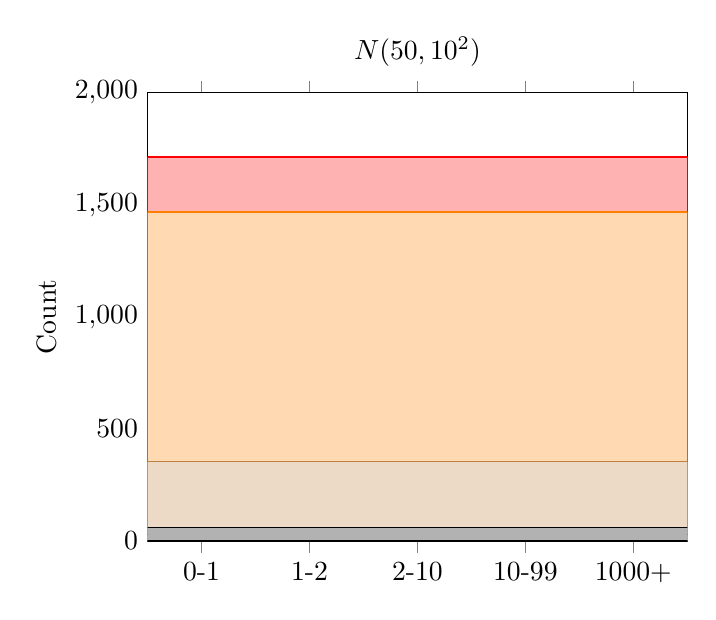
\begin{tikzpicture}
			\begin{axis}[
				x tick label style={draw=none},
				title={$N(50,10^2)$},
				%xlabel={Time (ms)},
				ylabel={Count},
				ybar,
				bar width=10,
				bar shift=0,
				xmin=0.5,
				xmax=5.5,
				ymin=0,
				ymax=2000,
				xtick={1,2,3,4,5},
				xticklabels={0-1,1-2,2-10,10-99,1000+}
				]
				\addplot[color=red,fill=red!30] coordinates {(1,1713)};
				\addplot[color=orange,fill=orange!30] coordinates {(2,1468)};
				\addplot[color=brown,fill=brown!30] coordinates {(3,353)};
				\addplot[color=blue,fill=blue!30] coordinates {(4,29)};
				\addplot[color=black,fill=black!30] coordinates {(5,62)};
			\end{axis}
		\end{tikzpicture}
		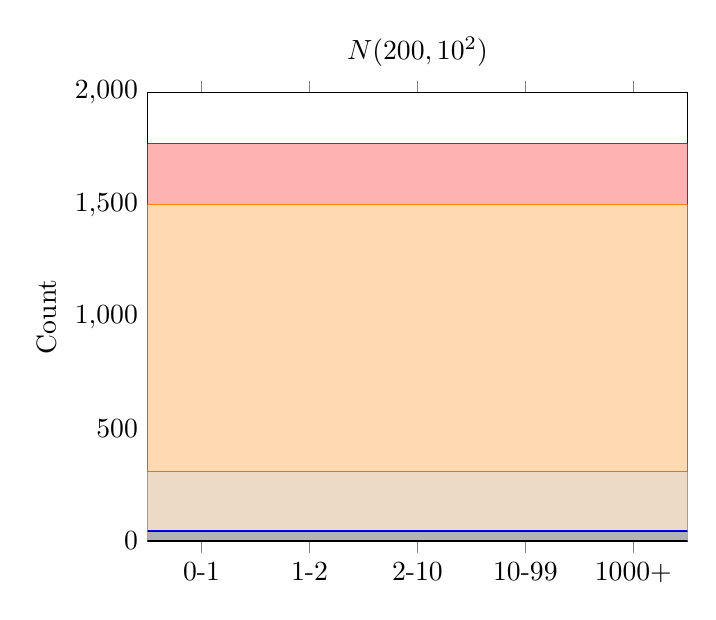
\begin{tikzpicture}
			\begin{axis}[
				x tick label style={draw=none},
				title={$N(200,10^2)$},
				%xlabel={Time (ms)},
				ylabel={Count},
				ybar,
				bar width=10,
				bar shift=0,
				xmin=0.5,
				xmax=5.5,
				ymin=0,
				ymax=2000,
				xtick={1,2,3,4,5},
				xticklabels={0-1,1-2,2-10,10-99,1000+}
				]
				\addplot[color=red,fill=red!30] coordinates {(1,1773)};
				\addplot[color=orange,fill=orange!30] coordinates {(2,1501)};
				\addplot[color=brown,fill=brown!30] coordinates {(3,309)};
				\addplot[color=blue,fill=blue!30] coordinates {(4,45)};
				\addplot[color=black,fill=black!30] coordinates {(5,44)};
			\end{axis}
		\end{tikzpicture}
		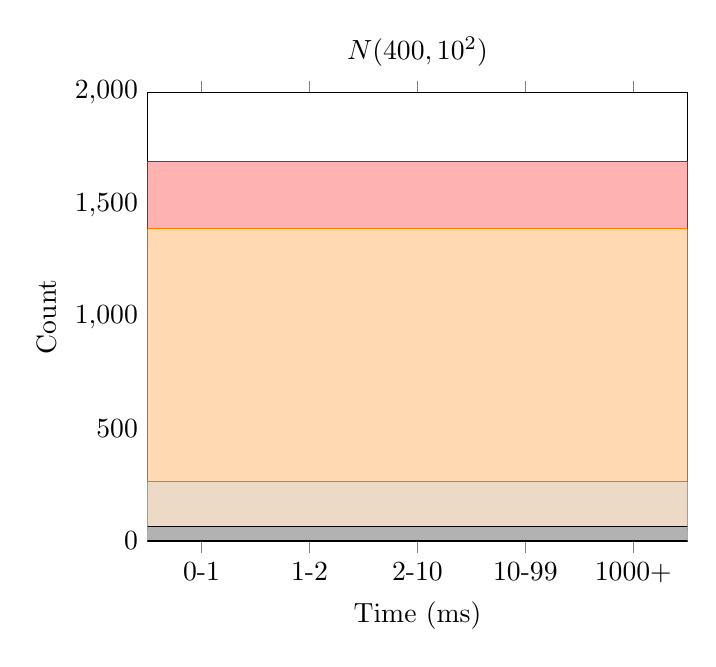
\begin{tikzpicture}
			\begin{axis}[
				x tick label style={draw=none},
				title={$N(400,10^2)$},
				xlabel={Time (ms)},
				ylabel={Count},
				ybar,
				bar width=10,
				bar shift=0,
				xmin=0.5,
				xmax=5.5,
				ymin=0,
				ymax=2000,
				xtick={1,2,3,4,5},
				xticklabels={0-1,1-2,2-10,10-99,1000+}
				]
				\addplot[color=red,fill=red!30] coordinates {(1,1694)};
				\addplot[color=orange,fill=orange!30] coordinates {(2,1394)};
				\addplot[color=brown,fill=brown!30] coordinates {(3,264)};
				\addplot[color=blue,fill=blue!30] coordinates {(4,51)};
				\addplot[color=black,fill=black!30] coordinates {(5,65)};
			\end{axis}
		\end{tikzpicture}
	\end{minipage}
	\hspace{-60pt}
	\begin{minipage}{0.48\textwidth}
		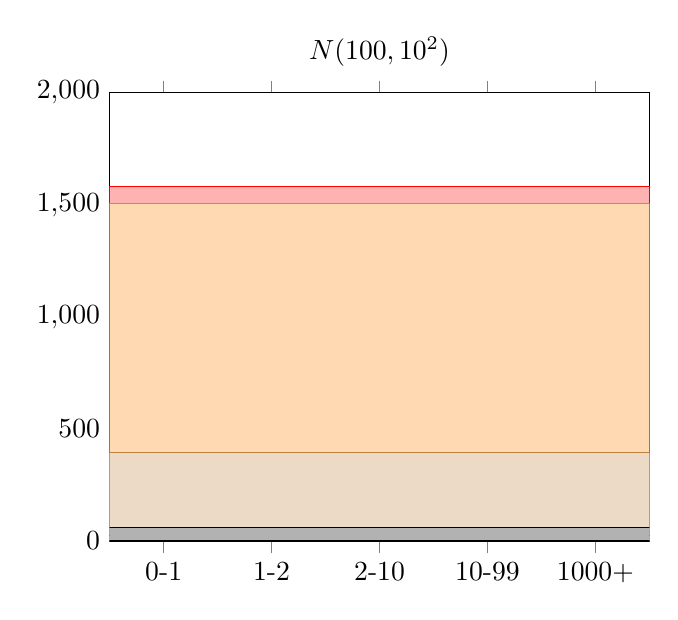
\begin{tikzpicture}
			\begin{axis}[
				x tick label style={draw=none},
				title={$N(100,10^2)$},
				%xlabel={Time (ms)},
				%ylabel={Count},
				ybar,
				bar width=10,
				bar shift=0,
				xmin=0.5,
				xmax=5.5,
				ymin=0,
				ymax=2000,
				xtick={1,2,3,4,5},
				xticklabels={0-1,1-2,2-10,10-99,1000+}
				]
				\addplot[color=red,fill=red!30] coordinates {(1,1582)};
				\addplot[color=orange,fill=orange!30] coordinates {(2,1506)};
				\addplot[color=brown,fill=brown!30] coordinates {(3,393)};
				\addplot[color=blue,fill=blue!30] coordinates {(4,24)};
				\addplot[color=black,fill=black!30] coordinates {(5,59)};
			\end{axis}
		\end{tikzpicture}
		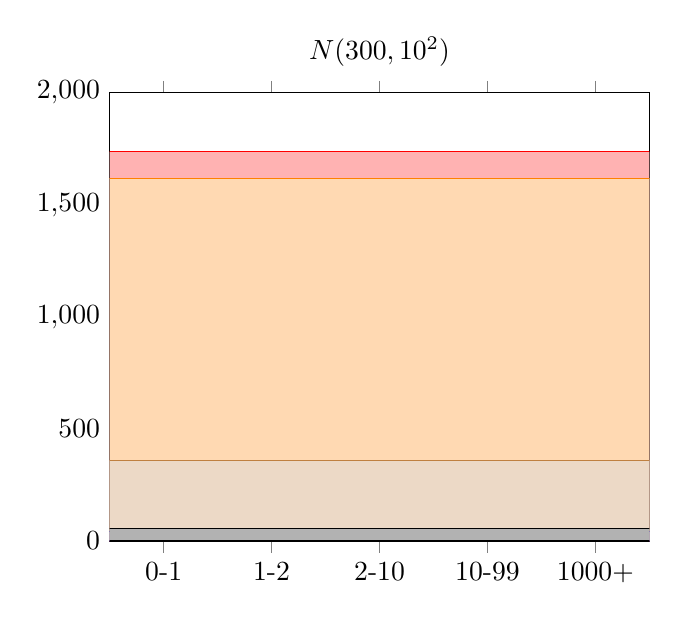
\begin{tikzpicture}
			\begin{axis}[
				x tick label style={draw=none},
				title={$N(300,10^2)$},
				%xlabel={Time (ms)},
				%ylabel={Count},
				ybar,
				bar width=10,
				bar shift=0,
				xmin=0.5,
				xmax=5.5,
				ymin=0,
				ymax=2000,
				xtick={1,2,3,4,5},
				xticklabels={0-1,1-2,2-10,10-99,1000+}
				]
				\addplot[color=red,fill=red!30] coordinates {(1,1736)};
				\addplot[color=orange,fill=orange!30] coordinates {(2,1619)};
				\addplot[color=brown,fill=brown!30] coordinates {(3,360)};
				\addplot[color=blue,fill=blue!30] coordinates {(4,42)};
				\addplot[color=black,fill=black!30] coordinates {(5,54)};
			\end{axis}
		\end{tikzpicture}
		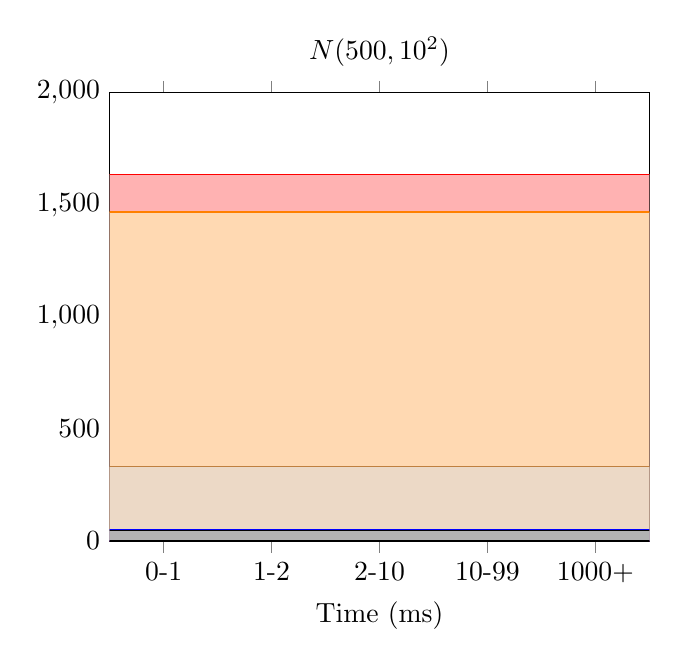
\begin{tikzpicture}
			\begin{axis}[
				x tick label style={draw=none},
				title={$N(500,10^2)$},
				xlabel={Time (ms)},
				%ylabel={Count},
				ybar,
				bar width=10,
				bar shift=0,
				xmin=0.5,
				xmax=5.5,
				ymin=0,
				ymax=2000,
				xtick={1,2,3,4,5},
				xticklabels={0-1,1-2,2-10,10-99,1000+}
				]
				\addplot[color=red,fill=red!30] coordinates {(1,1636)};
				\addplot[color=orange,fill=orange!30] coordinates {(2,1468)};
				\addplot[color=brown,fill=brown!30] coordinates {(3,332)};
				\addplot[color=blue,fill=blue!30] coordinates {(4,51)};
				\addplot[color=black,fill=black!30] coordinates {(5,46)};
			\end{axis}
		\end{tikzpicture}
	\end{minipage}
	\hspace{-80pt}
\end{document}